\section{KPMG on Low Code}\label{introduction-to-low-code-development}

I'm not sure which one of you is familiar with this new term, but it's
gaining a lot of attention globally. Although it may not be as popular
in Europe and Italy, there is another approach to software development
that is worth exploring. While technologies like that may be the current
trend, they are not the only ones that software engineers should focus
on in the next decade. There are new methods emerging that make software
development easier, faster, and more secure. Now, let's dive into the
details of low-code development, which is the topic we will be
discussing today.

\subsection{Definition and Scope}\label{definition-and-scope}

\begin{figure}[!h]
  \centering
  \includegraphics[page=7, trim = 2cm 2cm 2cm 0cm, clip, width=\imagewidth]{images/02 - KPMG_intelligent_automation_2.pdf}
\end{figure}

Low-code development is more than just a platform or a cloud solution.
It encompasses a combination of these elements. Now, let's move on
to discuss the major technologies involved in low-code development.

\subsection{Historical Context and
  Evolution}\label{historical-context-and-evolution}

Over the past decade, companies have
been increasingly focused on optimizing and streamlining their core
processes, such as procurement and operations. However, it's important
for companies to consider not only their core operations but also the
surrounding components that impact their overall efficiency. This
includes visualizing and automating common user tasks and leveraging
data to improve communication and collaboration with other departments.

In order to foster innovation, companies need to shift their attention
and resources towards individuals who can generate new ideas and
solutions. One common approach is to automate repetitive tasks or
non-value-added activities. This trend started years ago in large US
companies, including industrial giants like GM and banks, as well as
government institutions. Initially, the focus was on workforce
optimization rather than investment analysis. This was a simple and
straightforward solution at the time.

\subsection{Global Trends and
  Adoption}\label{global-trends-and-adoption}

In order to maintain our jobs and avoid outsourcing to
low-income countries like India, we need to take action. We can achieve
this by finding skilled individuals in these countries who can perform
our job effectively and at a lower cost. By doing so, we can reduce our
expenses and present a compelling case to management. This strategy is
commonly referred to as ``Outsourcing'' It is crucial for all
of us in the driving industry to understand and embrace this concept.

\subsection{Automation and Low-Code}\label{automation-and-low-code}

In these companies, there is a strong focus on automating activities
that were previously done by humans. This is the first aspect of
low-code development: automation. The idea behind this approach is to
find ways to automate these activities using robotic process automation
software. This technology is not new; it has been around for 14 years
and is commonly used in various applications. By implementing this
technology, companies can streamline their processes and reduce costs.

\subsection{Analytics and Data}\label{analytics-and-data}

The second aspect we will discuss is analytics. Analytics involves the
ability to analyze data collected from various sources within an
enterprise software system. It is important to create reports that not
only provide valuable insights but also optimize cost-effectiveness.
Analytics plays a crucial role in boosting automation. Automation relies
on both software and data, similar to how humans require data to perform
tasks efficiently. For instance, if a human needs to transfer data from
one window to another, they need the data to be organized and in a
suitable format. This ensures greater efficiency and effectiveness in
the overall process.

\subsection{Artificial Intelligence and
  Low-Code}\label{artificial-intelligence-and-low-code}

Lastly, but certainly not least, is the
application. Sometimes, you need tools to help you understand data and
make informed decisions, especially in automated processes. This is
where artificial intelligence (AI) comes into play. When AI intersects
with low-code development and automation, it creates a powerful
combination that can drive international competition.

\subsection{Low-Code as a Competitive
  Advantage}\label{low-code-as-a-competitive-advantage}

In the realm of international competition, the convergence of three key
elements---software, robotics, and business operations---is of utmost
importance. This combination allows for the creation of applications and
technologies that can significantly enhance business operations. One
notable advantage of this technology is its ability to automate crucial
tasks, resulting in increased efficiency. Moreover, the speed at which
these applications can be developed is truly remarkable. With this
technology, it is possible to create and deploy applications rapidly.

\subsection{The Future of Software
  Development}\label{the-future-of-software-development}

In the future, the landscape of software development will be drastically
different. Currently, companies rely on a large number of employees to
write code and build applications. However, with the advancements in
analytics, artificial intelligence, and automation, this process will be
revolutionized. These technologies will replace the need for manual
coding, making it much faster and more efficient.

As a result, the role of universities in teaching high-level programming
languages may become less important. The traditional approach to
software development will be replaced by low-code development, which
allows for faster and more streamlined application building. This means
that individuals who are currently studying programming may need to
reconsider their career paths, as the demand for manual coding skills
may decrease significantly in the next century.

It's important to embrace these changes and adapt to the future of
software development. By understanding the potential of low-code
development and the power of analytics, AI, and automation, individuals
can position themselves for success in this evolving industry.

\subsection{Low-Code Market Value}\label{low-code-market-value}

Why am I saying this? Because even today, if I want to develop a simple
enterprise application that requires some coding, I would
have needed to hire a Java or .NET programmer in the past. It would have
taken them around 10 to 20 days to complete the task. However, with
low-code development, I can do it myself in just one day. This
demonstrates the efficiency and time-saving benefits of low-code.

In the near future, I may not even need a person to configure the
low-code platform. Companies like Microsoft are continuously improving
their low-code tools, making them more user-friendly and accessible.
This evolution in low-code development is not just about individuals,
but it also has a significant impact on industries. Low-code has already
revolutionized billion-dollar infrastructures, not just small
businesses.

The global market value of low-code is currently around \$100 billion
per year, indicating a significant shift away from traditional
development methods.

\subsection{The Impact of Low-Code}\label{the-impact-of-low-code}

\subsubsection{Job Market and Industry
  Changes}\label{job-market-and-industry-changes}

My role here is to acknowledge a significant shift in the job market. In
my interviews with colleagues, I've encountered individuals who aspire
to be full-stack programmers, back-end developers, and content
developers. While these roles are valuable, it's important to recognize
that they may become less prevalent in the future. Companies like ours, have chosen to focus on the strength of technology rather
than relying on a large number of developers spread across the globe. We
have witnessed the growing importance and popularity of technologies
like cybersecurity and bandwidth growth. This is why we have made the
decision to invest in these technologies and share this information with
you.

\subsubsection{The Role of Traditional Software
  Development}\label{the-role-of-traditional-software-development}

I understand your concerns about your ability to excel in your job and
the challenges you face in the software industry. It can be difficult
when there is a lack of resources and support. However, it's important
to remember that the industry is constantly evolving, and there are new
opportunities emerging.

One such opportunity is low-code development, which allows individuals
without extensive coding experience to create applications. Low-code
platforms provide a visual interface and pre-built components that
simplify the development process. This means that even if you don't
consider yourself a skilled engineer, you can still contribute to
software development.

The rise of low-code development has also led to increased automation in
the industry. Tasks that were once time-consuming and manual can now be
automated, freeing up valuable time for more complex work. This
automation is particularly beneficial in the front-end development
space, where there is often a shortage of skilled individuals.

However, it's important to acknowledge that the traditional software
development industry is still relevant and necessary. While low-code
development offers advantages, there are still complex projects that
require the expertise of experienced engineers. It's about finding the
right balance and leveraging the strengths of both approaches.

In conclusion, the software industry is evolving, and low-code
development is becoming a competitive advantage. It provides
opportunities for individuals without extensive coding backgrounds and
enables automation in the development process. However, traditional
software development still plays a crucial role in tackling complex
projects. It's important to adapt to these changes and embrace new
technologies to stay relevant in the industry.

\subsubsection{New Opportunities in Software
  Industry}\label{new-opportunities-in-software-industry}

There is a new and rapidly growing software industry that is gaining
momentum. It may seem like a small trend, but it has actually been
developing for the past 20 to 30 years. Initially, there were only a few
companies involved, but now there are countless players in the market.
These companies are often overshadowed by larger, more well-known
organizations, but they are making significant contributions in various
sectors, including healthcare and media.

The emergence of this new software industry has created numerous job
opportunities, but there is a shortage of skilled professionals who are
familiar with the technology. One reason for this shortage is that many
people are not yet aware of the potential of this industry.
Additionally, traditional software developers may be hesitant to
transition to this new field.

However, it is important to recognize the potential and embrace the
changes that this industry brings. It offers exciting prospects and
opens up new avenues for innovation. It's time to break away from
traditional norms and explore the possibilities that this new software
industry has to offer.

\subsection{Low-Code in Practice}\label{low-code-in-practice}

\subsubsection{Intelligent Automation}\label{intelligent-automation}

So, returning to our presentation, these are the tasks that
someone working in intelligent automation can perform. It's not just
about developing solutions; it involves IT professionals engaging in a
wider range of activities. It's not like being a software developer,
where you gather requirements, develop an application, and then test and
deploy it. In intelligent automation, we also have the task of
discovery. We engage in value-added activities to understand how
automation can be applied to companies, build those automation
solutions, and incorporate elements of cognitive and artificial
intelligence. And, ultimately, we also handle management. Let me provide
an example. One of our projects serves as a very interesting use case.

\subsubsection{Use Cases and Efficiency}\label{use-cases-and-efficiency}

For an automotive company that increased its production of luxury cars,
there was a challenge related to checking the labels on each vehicle.
These labels contain important information, such as the manufacturing
location and pressure specifications, and must comply with local
regulations and be in the language of the market where the car is sold.
Previously, employees on the production line manually checked each label
for accuracy and compliance.

To address this issue, a discovery process was conducted to identify
opportunities for automation. A solution was developed using a
combination of low-code development, cognitive technology, and
artificial intelligence. An app was created for tablets used by the
employees on the production line. They could simply take a picture of
the labels on the car doors and other locations, and an Amazon Web
Service configured with label recognition capabilities would
automatically analyze the image. The system would determine if the label
was correct, in the right position, and compliant with regulations. The
results were recorded and archived in the tool.

By implementing this automated solution, the automotive company was able
to reduce the number of employees needed for label checking from five to
just a couple. This resulted in significant cost savings for the
company.

\subsubsection{Tools and Technologies}\label{tools-and-technologies}

At our company, we go beyond just being software engineers. We strive to
find the best solutions and automation techniques to add value to our
clients' businesses. We use various tools, such as Microsoft, AWS, and
others, to create high-level architectures for automating human
activities. One of the tools we use is Robotic Process Automation (RPA),
which allows us to automate repetitive tasks. We also utilize HR and
cognitive services, as well as low-code development, to build
applications. Think of us as painters who combine different technologies
to automate work processes. This approach is incredibly powerful and
transformative.

\subsubsection{Traditional vs.~Low-Code
  Development}\label{traditional-vs.-low-code-development}

If we look back 10 or 20 years ago, the only option for software
development was writing code in specific programming languages like .NET
or C\#. However, today we have a wider range of technologies
available to us. This has led to the emergence of low-code development.

Traditional development is a manual process carried out by humans, which
can be prone to errors and requires significant resources. Developers
often spend a lot of time searching for code, trying to understand it,
and sometimes making mistakes that require further investigation. On the
other hand, low-code development offers a different approach.

With low-code, developers have access to a palette of pre-built
components and services that can be reused. Many of these components
have already been created by other developers, allowing for efficient
reuse of their work. This is the essence of low-code development: the
ability to create applications without having to write traditional code.

\subsection{The Future of Low-Code}\label{the-future-of-low-code}

\subsubsection{Predictions and Market
  Trends}\label{predictions-and-market-trends}

Low-code development is gaining popularity due to its ease of use and
ability to bridge the gap between business needs and software
development. Compared to traditional software development, low-code
allows for faster results and the ability to showcase them more quickly.
This is particularly important because by 2025, the majority of
enterprise application development is expected to be done using
low-code. This shift towards low-code presents a significant opportunity
for industries to adopt this approach. The low-code market is projected
to reach \$30 billion by 2025, making it crucial for businesses to
embrace this trend and stay competitive.

\subsubsection{Digital Solutions and Legacy
  Modernization}\label{digital-solutions-and-legacy-modernization}

Low-code development offers a range of possibilities for various
applications. One key benefit is the ability to create new digital
solutions that can be used both internally and externally. These
solutions can be utilized by employees within the company as well as by
consumers who want to interact with the organization.

Another valuable use of low-code is the modernization of legacy
applications. Many industries, such as banking, still rely on outdated
applications developed in the 70s or 80s. With low-code, companies can
transition these old technologies to more modern platforms by developing
low-code applications.

Additionally, low-code can be used to streamline and consolidate
applications across different departments. In the past, companies would
build separate applications for each department, resulting in a lack of
cohesion. Low-code allows for the unification of these applications into
a single, integrated system.

Lastly, low-code enables the automation and orchestration of existing
processes, as well as the design of new processes. This means that
companies can automate repetitive tasks and workflows, improving
efficiency and productivity.

These four areas---creating new digital solutions, modernizing legacy
applications, unifying applications across departments, and automating
processes---are the primary use cases for low-code development.

\subsubsection{Low-Code Landscape}\label{low-code-landscape}

\begin{figure}[!h]
  \centering
  \includegraphics[page=14, trim = 2cm 2cm 2cm 0cm, clip, width=\imagewidth]{images/02 - KPMG_intelligent_automation_2.pdf}
\end{figure}

\begin{figure}[!h]
  \centering
  \includegraphics[page=15, trim = 2cm 2cm 2cm 0cm, clip, width=\imagewidth]{images/02 - KPMG_intelligent_automation_2.pdf}
\end{figure}

In the landscape of low-code development, there are different types of
applications that can be built. One example is multi-experience
platforms, which allow you to develop applications that can be deployed
on mobile devices, tablets, or web browsers. These platforms focus on
providing a seamless user experience across different devices.

Another type of platform is functional extension platforms. These
platforms are used to enhance existing enterprise software by
configuring and augmenting processes. They enable businesses to extend
the functionality of their software without the need for extensive
coding.

For those who are new to coding or prefer a more user-friendly approach,
there are citizen developer platforms. These platforms require no coding
knowledge and are designed to be easy to use for anyone, including
non-technical individuals. They are often used by companies to create
small-scale applications quickly and efficiently.

Lastly, there are business process management platforms. These platforms
are used to digitize complex processes within organizations. By
leveraging these technologies, businesses can develop solutions that
streamline and automate intricate processes.

Overall, the low-code landscape offers a range of platforms tailored to
different application development needs, from multi-experience platforms
to functional extension platforms, citizen developer platforms, and
business process management platforms.

\subsection{Hands-On Exercise}\label{hands-on-exercise}

\subsubsection{Design Activity and User
  Experience}\label{design-activity-and-user-experience}

Low-code development can be used in various scenarios, such as digital
transformation initiatives, workflow automation, creating specialized
software for niche industries where enterprise software is not
available, and modernizing legacy systems. The versatility of low-code
allows for a wide range of applications.

For today's exercise, we will focus on a low-code platform and simulate
a project similar to what we do in real-life low-code projects. One of
the initial phases in a low-code project is the design activity. During
this phase, we need to consider the process, the data involved, the
users of the application, and the user interface.

Designing a user interface is a complex task in today's world. We need
to develop applications that are easy to use for everyone and accessible
across multiple devices. Low-code software can assist in this process by
providing a palette of optimized graphic layouts for mobile, laptop, and
public use. However, creating a user interface that meets these
requirements remains challenging.

For today's exercise, we will focus on user experience (UX) and user
interface design (UI).

\subsubsection{ACME Company Case Study}\label{acme-company-case-study}

\begin{figure}[!h]
  \centering
  \includegraphics[page=17, trim = 2cm 2cm 2cm 0cm, clip, width=\imagewidth]{images/02 - KPMG_intelligent_automation_2.pdf}
\end{figure}

ACME, a company, has approached us to develop a workforce time report. A
time report is essentially a calendar where individuals working on
projects or for a company can log their time. They record the number of
hours spent on specific tasks, such as training, project work, or email
responses. ACME has requested us to design the entire solution,
including the user interface.

When it comes to the user interface, our usual approach is to create a
wireframe. A wireframe is a sketch of the user experience that takes
into account the technical requirements of IT software. It needs to be
compatible with webpages, easy to use, and mobile-friendly. Designing a
user experience is a complex task that requires careful consideration.

To facilitate this process, we recommend using a tool like \href{https://www.drawio.com}{Draw.io}. It
allows us to create detailed wireframes that align with ACME's needs and
preferences. By collaborating as a group, we can ensure that the final
design meets all the necessary criteria for a successful workforce time
report.

\subsubsection{Success Criteria and Business
  Rules}\label{success-criteria-and-business-rules}

One of the free tools available on the web for building a user
experience is wireframing. While you can use PowerPoint, I strongly
recommend using a tool specifically designed for this purpose. To create
the wireframes for ACME Company, we need to start with an on-page for
the employee. As an employee, I would need to enter my username and
password, and there could also be additional authorization steps such as
multi-factor authentication or a one-time password. We also want to
include navigation to the time report page and an expense report page.

The expense report page is where employees can enter their expenses,
such as travel expenses. This page should allow users to input details
about the expense, including the date, type, receipt upload, amount, and
location. It's important to consider all the necessary information for
expense reporting.

When designing the wireframes, it's crucial to keep in mind the success
criteria. As consultants, we are always evaluated based on these
criteria. One important aspect is the navigation between pages. It's
common for teams to focus on designing beautiful pages but overlook the
seamless transition between them. Users should be able to easily
navigate back and forth between pages, as mistakes can happen during
data entry.

Another consideration is the user interface (UI). Avoid using large
white boxes on a page, as this can be a common mistake. Just like you as
a consumer wouldn't appreciate a lackluster UI on your iPhone or
Android, it's important to judge your own design from a user's
perspective. Additionally, it's essential to define the business rules
behind each page. These rules will guide the functionality and behavior
of the application.

By taking these factors into account and creating wireframes that
prioritize user experience, navigation, and a visually appealing UI, we
can ensure the success of the ACME Company application.

\subsection{Closing Remarks and Exercise
  Instructions}\label{closing-remarks-and-exercise-instructions}

For example, let's consider a validation process. It's important to
ensure that expenses are only entered for the days worked. Keep in mind
that these validations are not optional---they are necessary.
Additionally, it's crucial to make sure that the user interface (UI) is
responsive and adaptable to different devices. Instead of relying on
adjusting the power pointer, it's recommended to utilize the UI, which
is accessible across all devices. Remember, we are not just focusing on
time, but also on expenses. It's important to consider the user
experience and not overlook the needs of the users. Lastly, building
security is essential. An authentication mechanism should be implemented
to protect sensitive data. This exercise is designed to help you
understand the group's requirements. Since there is a lot of work to be
done and a meeting scheduled for later this afternoon, it would be
beneficial for you to start working on it now.
